\section{Abridged 2015-05-29 Product Manager Interview}

\textbf{Todd:} This is a drawing exercise for you. So, pretty open-ended question, could you describe a project work flow by drawing it on that sheet of paper? There's no wrong answers. 02:32

\begin{figure}[h]
\centering
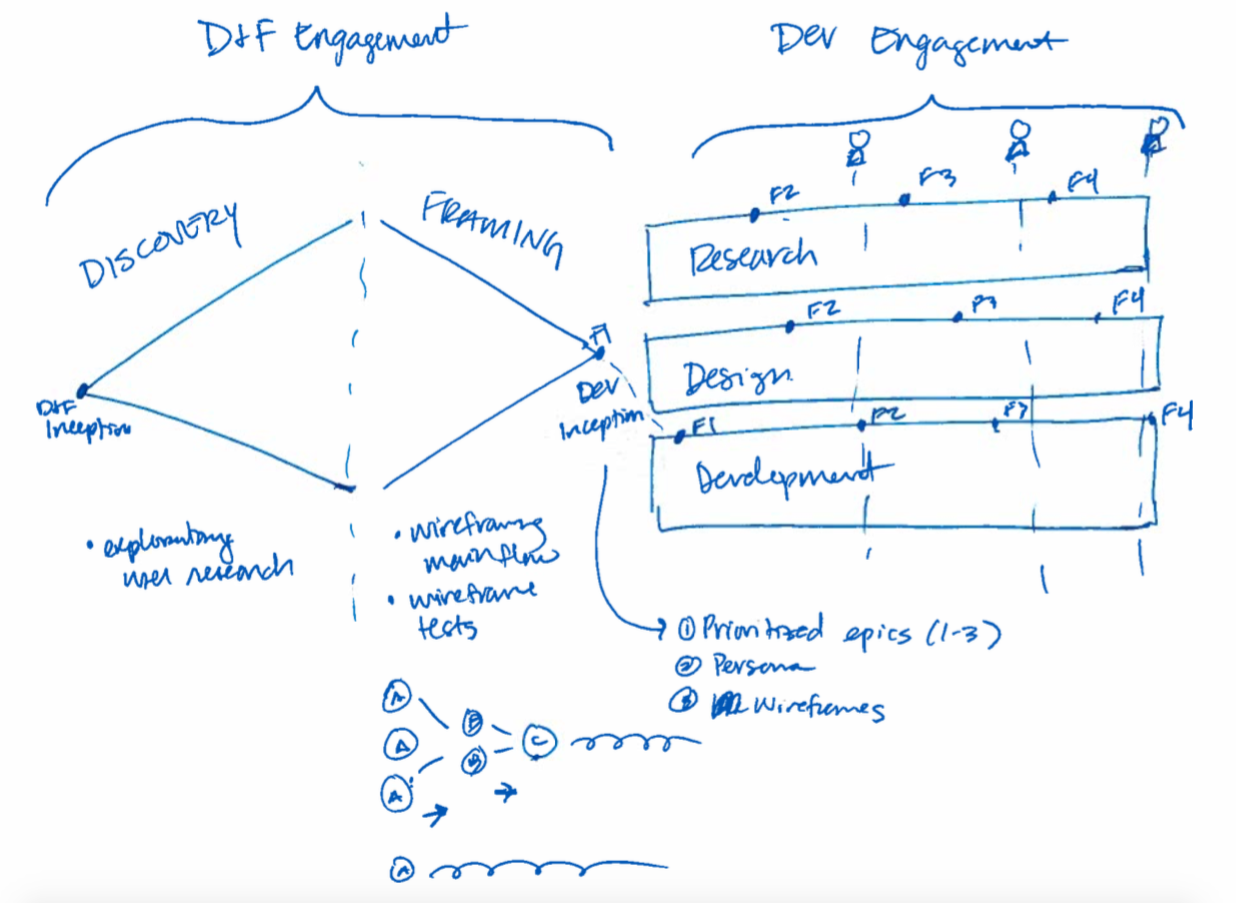
\includegraphics[width=6.5in]{interviews/drawings/2015_05_29.png}
\caption{\quotes{2015-05-29's drawing of a project work flow}}
\label{2015_05_29}
\end{figure}

\textbf{Interviewee:} Does it matter if there's a DNF first or...? 02:39

\textbf{Todd:} However you want it. Typical, ideal, however you want to draw it. 02:44

\textbf{Interviewee:} We actually show this to clients. We have this drawing here. 02:54

\textbf{Interviewee:} Most of the projects that I've been on start with the DNF. We'll call this DNF. 03:07

\textbf{Interviewee:} It's assuming the project has design in development going. This kind of, like, inception. 03:27

\textbf{Interviewee:} And this is dev inception. 03:32

\textbf{Interviewee:} This is your discovery, and framing. 03:50

\textbf{Interviewee:} Here in this area, we're sort of doing more exploratory research and sort of going wide trying to understand the users. That's something we do at the beginning of every project especially if the client doesn't know who their user is or they have ideas of who they are but it's not validated. 04:10

\textbf{Todd:} 	That's the discovery phase. 04:11

\textbf{Interviewee:} Yes. So, this is like exploratory user research. That's like interviews and maybe on site, shadowing people and things like that. And once we have a good idea of who they are, we start wire framing, maybe like the main flow and doing some wire frame tests like user research, that kind of thing and that's kind of within that, I think, we're kind of iterating as well. 04:45

\textbf{Interviewee:} I guess you can either start with one and iterate on that or you can start with many and narrow down. We've done both. So, when you start with many, you just- So, this is like your different As, research, then research to get to C. That makes sense? 05:10

\textbf{Todd:} It's like a portfolio of ideas? 05:14

\textbf{Interviewee:} Yes. I did it on my first project and it worked out really well and then from there you're kind of iterating on what you've come up with. 05:25

\textbf{Interviewee:} We came up with a couple, different nuance ways of doing something because they all seem good and they're like, two or three different features and we sort of combined them in different ways and then we took our insights from that and narrowed it down two versions, narrowed it down to one version. 05:46

\textbf{Interviewee:} I've also done it where you just start with A and you just iterate. I think both worked but this is fun to do. By the time we get to dev inception, we have prioritized epics. You have a develop persona. And you have wire frames. That's kind of the ideal for this point. At that point, development can start on say feature one and in the meantime, we'll start researching feature two. Then, we'll develop it. Then, feature three. So, it kind of goes like that. 06:37

\textbf{Todd:} Nice. 06:39

\textbf{Interviewee:} Maybe you have feature one here and then we'll go here. While they're doing that, we'll start on the next thing. So, on the next thing it flows down. I hate saying waterfall because I know it's the wrong kind. It's like a different kind of waterfall but it iterates in that way. So, we're like, \quotes{Oh, it's going in the cycle.} At any time, we're going to bring in users to test whatever we want. 07:09

\textbf{Todd:} You're drawing people. 07:12

\textbf{Interviewee:} Yes. These are users. At any given point, we can even do exploratory research. We can do wire frame or visual research or we can show them an actual prototype. 	It's kind of nice because you can, whenever you need people, whenever you're stuck on something, you don't have to wait for the right time to bring people in. 	It's just you can test anything at any given time.  07:34
